% docker run --rm -it -v $(pwd):/home danteev/texlive latexmk -pdf document.tex
% https://en.wikibooks.org/wiki/LaTeX
% https://ctan.org/tex-archive/info/lshort/english/

%\documentclass[11pt, a4paper]{article}
\documentclass[12pt, a5paper]{book}
\usepackage[a5paper]{geometry}
%\usepackage[paperwidth=5.5in, paperheight=8.5in]{geometry}
\usepackage[utf8]{inputenc}
\usepackage{graphicx}
\usepackage{hyperref}
%\usepackage[default]{lato}
\usepackage[T1]{fontenc}
\usepackage[german,ngerman]{babel}
\usepackage[right]{eurosym}
\usepackage[bottom]{footmisc}
\usepackage{blindtext}

\date{}
\begin{document}

\title{\textbf{Willkommen bei \LaTeX}}
\author{Marcus Baer}

\maketitle

\chapter{Der Anfang mit \LaTeX}

\section{Der Anfang mit \LaTeX}

Hier beginnt nun unser erstes wunderbares \LaTeX-Dokument\footnote{Eine Dokumentation von {\LaTeX} findet sich \href{https://en.wikibooks.org/wiki/LaTeX}{in diesem Wiki}, eine nicht so kurze \href{https://ctan.org/tex-archive/info/lshort/english/}{bei CTAN}.},
das die \textsl{grundlegenden} Eingaben zeigen soll ohne Detailstaffelei \dots

Abbildung \ref{fig:autor} zeigt den \emph{Autor} des Dokuments auf Seite \pageref{fig:autor}.

\begin{itemize}
\item \blindtext
\begin{enumerate}
\item Nested item 1
\item Nested item 2
\end{enumerate}
\item \blindtext
\end{itemize}

\begin{figure}
  \centering
    %\write18{wget http://www.some-site.com/path/to/image.png}
    %\includegraphics[width=0.5\textwidth]{image.png}
    %\includegraphics[width=0.5\textwidth]{gull}
    \href{http://www.marcusbaer.info}{
        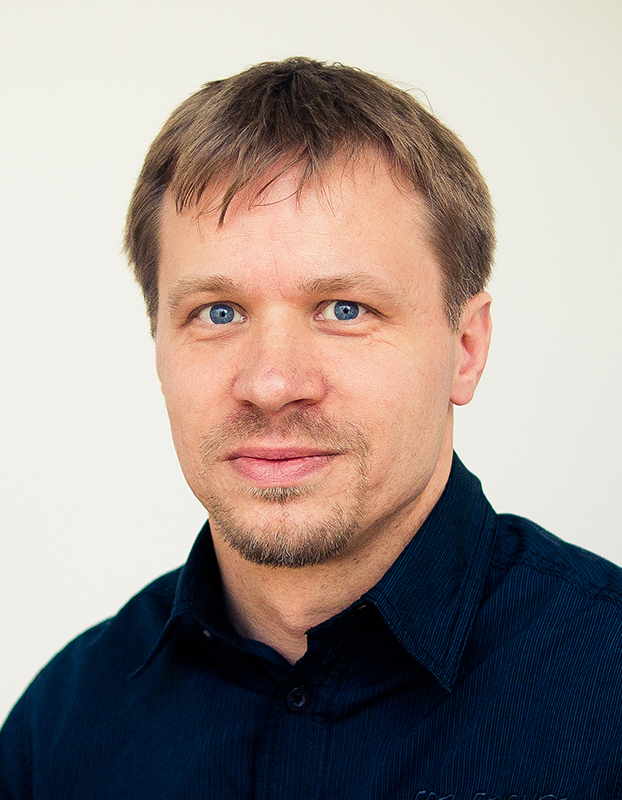
\includegraphics[width=0.5\textwidth]{Marcus}
    }
    \caption{Der Autor des Dokumentes}
    \label{fig:autor}
\end{figure}

\begin{figure}
  \centering
    
\includegraphics[width=0.5\textwidth]{Docker.png}
    \caption{Logo von Docker}
    \label{fig:logo}
\end{figure}

\begin{table}
  \centering
    \begin{tabular}{| l | c | r |}
    \hline
    1 & 2 & 3 \\[5mm] \hline
    4 & 5 & 6 \\ \hline
    7 & 8 & 9 \\
    \hline
    \end{tabular}
  \caption{Eine einfache Tabelle}
\end{table}

\end{document}

% \documentclass[12pt]{article}
% \usepackage{tasks}
% \usepackage{exsheets}
% \SetupExSheets[question]{type=exam}
% \begin{document}
% \begin{question}
% 	Which one of the entries does not fit with the others?
% 	\begin{tasks}(4)
% 		\task mercury
% 		\task iron
% 		\task lead
% 		\task zinc
% 	\end{tasks}
% \end{question}
% \settasks{
% 	counter-format=(tsk[r]),
% 	label-width=4ex
% }
%\begin{question}
%	What is a funkyton?
%	\begin{tasks}(2)
%		\task A dancing electron
%		\task A dancing proton
%		\task A dancing neutron
%		\task A Dixie Dancing Duck
%	\end{tasks}
%\end{question}
%\end{document}

% INSPIRATION
% http://songs.sourceforge.net/